\chapter{Evaluation}
\label{ch:evaluation}

In this chapter we present the evaluation of the methods proposed in the previous part, chapter~\ref{ch:reducing}. These models were tested in terms of speed and accuracy. The data sets selected for evaluation vary both as number of samples~$N$ and as dimensionality~$D$, table~\ref{tab:datasets}. The diversity of the data sets made assessing the performance of the algorithms difficult. It is known that there is no free lunch in accurately solving widely different problems.

For evaluation we used $70\%$ of the data set for training and the rest of $30\%$ was kept for testing. We made exceptions for two data sets: \texttt{landsat} and \texttt{mnist}. These are commonly already split in training and testing sets.

We started testing NCA on small data sets. This allowed us to have a baseline to compare the new models against, table \ref{table:eval-baseline}. This can also be viewed as a replication of the work in the original article \citet{goldberger2004}. The authors did not provide us with information about their implementation. For this series of experiments, we used random initialization and we optimized the function using conjugate gradients. The results are averaged over 40 runs. We also considered the score obtained in the original space. We computed this using leave one out cross validation using the Euclidean metric. The results are quite similar to those presented in the original paper.  

However, in order to achieve a robust implementation of NCA we had to carry out additional experiments. The learnt lessons were summarized in section~\ref{sec:practical-notes}. We will see the influence of the implementation tricks in the following results, section~\ref{sec:method-comparison}. Additional results are attached at the end of the thesis, appendix~\ref{app:results}:
\begin{itemize}
 \item Tables~\ref{table:comp-opts-1} and~\ref{table:comp-opts-2} presents a compares two possible optimization methods for NCA: conjugate gradients and gradient ascent with ``bold driver'' heuristic.
 \item Figures~\ref{fig:iris-init}, \ref{fig:balance-init} and~\ref{fig:ecoli-init} illustrate the initialization effect. 
\end{itemize}

% 
% \section{Setup}
% \label{sec:setup}

% The functions were implemented in \texttt{MATLAB} and are the author's own work. Some other functions that were.

\begin{table}%
  \centering
    \begin{tabular}{l l c c c} \toprule
	Data set name&Abbrevation&$N$&$D$&$C$\\ 
	\midrule
	Balance scale&\texttt{balance}&$625$&$4$&$3$\\ 
	Ecoli&\texttt{ecoli}&$336$&$7$&$8$\\ 
% 	&\texttt{fruit}&$59$&$3$&$3$\\ 
	Glass identification&\texttt{glass}&$214$&$9$&$6$\\ 
	Ionosphere&\texttt{ionosphere}&$351$&$33$&$2$\\ 
	Iris&\texttt{iris}&$150$&$4$&$3$\\ 
	Landsat satellite&\texttt{landsat}&$6435$&$36$&$6$\\ 
	MAGIC Gamma telescope&\texttt{magic}&$19020$&$10$&$2$\\ 
	MNIST digits&\texttt{mnist}&$70000$&$784$&$10$\\ 
% 	&\texttt{olivetti}&$400$&$4096$&$40$\\ 
	Pima Indians diabetes&\texttt{pima}&$768$&$8$&$2$\\ 
	Image segmentation&\texttt{segment}&$2310$&$18$&$7$\\ 
	SPECTF heart&\texttt{spectf}&$267$&$44$&$2$\\ 
	Blood transfusion&\texttt{transfusion}&$748$&$4$&$2$\\ 
	USPS digits&\texttt{usps}&$11000$&$256$&$10$\\ 
	Wine&\texttt{wine}&$178$&$13$&$3$\\ 
	Yeast&\texttt{yeast}&$1484$&$8$&$10$\\  
      \bottomrule
    \end{tabular}
\caption{\small \small This table presents the characteristics of the data sets used: number of samples $N$, dimensionality of the data $D$ and number of classes $C$. The two digits data sets \texttt{mnist} and \texttt{usps} were downloaded from the following URL \protect\url{http://cs.nyu.edu/~roweis/data.html}. All the others data sets are available in the UCI repository \protect\url{http://archive.ics.uci.edu/ml/datasets.html}.}
\label{tab:datasets}
\end{table}

\begin{table}
  \centering\begin{tabular}{lrcccc}
  \toprule
	  &     & Train score  & \multicolumn{2}{c}{Test scores} & Baseline \\
  \cmidrule(r){3-3} \cmidrule(r){4-5} \cmidrule(r){6-6}
  Data set & $d$ & $f(A)$ & $1$-NN & NCA & Eucl. \\
  \midrule
    \texttt{balance}&$2$&$92.86 \pm 0.47$&$90.78 \pm 0.53$&$90.61 \pm 0.55$&\\ 
		    &$D=4$&$95.36 \pm 0.38$&$93.40 \pm 0.47$&$93.04 \pm 0.51$&$76.18$\\ 
    \midrule
    \texttt{ionosphere}&$2$&$98.31 \pm 0.14$&$79.86 \pm 0.75$&$79.74 \pm 0.78$&\\ 
		       &$D=33$&$72.07 \pm 0.71$&$86.22 \pm 0.64$&$72.87 \pm 0.71$&$85.38$\\ 
    \midrule
    \texttt{iris}&$2$&$99.38 \pm 0.11$&$94.94 \pm 0.39$&$94.72 \pm 0.39$&\\ 
		 &$D=4$&$99.48 \pm 0.10$&$95.10 \pm 0.44$&$95.15 \pm 0.44$&$95.53$\\
    \midrule
    \texttt{wine}&$2$&$99.15 \pm 0.14$&$92.4 \pm 1.0$&$92.4 \pm 1.0$&\\ 
		 &$D=13$&$98.95 \pm 0.15$&$95.36 \pm 0.51$&$95.36 \pm 0.51$&$74.53$\\ 
  \bottomrule
  \end{tabular}
  \caption{\small Accuracy of standard NCA on four small data sets. Scores are averaged over 40 runs. The second column presents the dimensionality~$d$ the data set is reduced to. The last column shows the leave one out cross validation performance on the data set using Euclidean metric.}
  \label{table:eval-baseline}
\end{table}

\section{Mini-batches methods comparison}
\label{sec:method-comparison}

First we present individual results for each of the methods. We also give details about the methodology and the parameter choices. The final comparison is illustrated at the end of this subsection using an error \textit{vs.} time representation.

The methods were compared in this section on the top 3 largest data sets as number of points $N$.

\begin{description}
  \item[Subsampling.] {
    For this method we trained NCA on a subset of $n=3000$ samples. We used conjugate gradients for optimization and for initialization RCA linear transformation. We observe that the training scores are significantly better than the train performance, especially on \texttt{usps} data set. As previously mentioned, the thinning effect is a cause for this.
    \begin{table}
    	\centering
    	\begin{tabular}{lccc}
    	\toprule
    	Data set & Train & $1$NN & NCA \\
    	\cmidrule(r){2-2}\cmidrule(r){3-3}\cmidrule(r){4-4} 
    	 \texttt{usps}&$99.112 \pm 0.099$&$89.30 \pm 0.18$&$89.41 \pm 0.16$\\
    	 \texttt{magic}&$82.71 \pm 0.41$&$79.25 \pm 0.45$&$80.22 \pm 0.72$\\
    	 \texttt{mnist}&$96.867$&$82.130$&$82.470$\\
    	 \bottomrule
    	\end{tabular}
    \end{table}
  }
  \item[Mini-batches.] {
    To get significant gradients we used large mini-batches $n=2000$. The points in a batch are selected via recursive projection clustering (RPC) algorithm. We trained the metric using gradient ascent with early stopping. The learning rate had a the form $\frac{\eta}{t+t_0}$. We fixed $\eta=1$ and tuned parameter $t_0$ using cross validation across an exponential scale; also finer tuning is done across a linear scale. We used $5\%$ of the training set for cross validation and we  monitor the accuracy on the cross validation set at each iteration. If the performance does not increase for $25$ iterations, we stop the learning process. 
    \begin{table}
        	\centering
        	\begin{tabular}{lccc}
        	\toprule
        	Data set & Train & $1$NN & NCA \\
        	\cmidrule(r){2-2}\cmidrule(r){3-3}\cmidrule(r){4-4} 
        	 \texttt{usps}&$92.00 \pm 0.43$&$91.26 \pm 0.17$&$92.37 \pm 0.17$\\
        	 \texttt{magic}&$80.04 \pm 0.48$&$79.14 \pm 0.52$&$79.8 \pm 1.1$\\
        	 \texttt{mnist}&$87.47 \pm 0.49$&$87.52 \pm 0.36$&$89.88 \pm 0.25$\\
        	 \bottomrule
        	\end{tabular}
    \end{table}
    
  }
  \item[Stochastic learning.] {
    We considered $n=50$ neighbours to look at for each iteration. The learning procedure is similar to the one applied for the mini-batches method: gradient ascent with early stopping. The same observation as before apply here. 

    Besides the results on the large data sets, we also present the performance of this method when used for small data sets. We mostly observe similar results as the baseline NCA. The most significant difference is that the classification done using NCA objective function is better than $1$NN classification.

    \begin{table}
      \centering\begin{tabular}{lrccc}
      \toprule
	      &     & Train score  & \multicolumn{2}{c}{Test scores}\\
      \cmidrule(r){3-3} \cmidrule(r){4-5}
      Data set & $d$ & $f(A)$ & $1$-NN & NCA \\
      \midrule
	\texttt{balance}&$2$&$88.35 \pm 0.83$&$87.37 \pm 0.49$&$90.45 \pm 0.38$\\  
	&$D=4$&$94.70 \pm 0.87$&$95.32 \pm 0.34$&$96.14 \pm 0.29$\\ 
	\midrule
	\texttt{ionosphere}&$2$&$89.0 \pm 1.7$&$85.71 \pm 0.94$&$87.08 \pm 0.95$\\
	&$D=33$&$92.6 \pm 1.5$&$84.72 \pm 0.57$&$84.34 \pm 0.59$\\ 
	\midrule
	\texttt{iris}&$2$&$96.41 \pm 0.94$&$96.33 \pm 0.57$&$97.00 \pm 0.46$\\ 
	&$D=4$&$97.5 \pm 1.3$&$95.67 \pm 0.71$&$96.11 \pm 0.66$\\ 
	\midrule
	\texttt{wine}&$2$&$98.80 \pm 0.70$&$97.22 \pm 0.65$&$97.50 \pm 0.49$\\ 
	&$D=13$&$99.25 \pm 0.62$&$96.85 \pm 0.41$&$96.85 \pm 0.41$\\ 
      \bottomrule
      \end{tabular}
      \caption{\small Stochastic NCA results on small data sets.}
    \end{table}
        \begin{table}
            	\centering
            	\begin{tabular}{lccc}
            	\toprule
            	Data set & Train & $1$NN & NCA \\
            	\cmidrule(r){2-2}\cmidrule(r){3-3}\cmidrule(r){4-4} 
            	\texttt{usps}&$90.23  \pm 0.50$&$90.68 \pm 0.22$&$92.64 \pm 0.17$\\
            	\texttt{magic}&$78.39 \pm 0.25$&$79.76 \pm 0.13$&$84.49 \pm 0.12$\\
            	\texttt{mnist}&$85.97 \pm 0.37$&$86.07 \pm 0.43$&$89.35 \pm 0.39$\\
            	
            	 \bottomrule
            	\end{tabular}
        \end{table}
    }
\end{description}
\begin{figure}
	  \centering
	  \subfigure[\texttt{usps}]{\label{fig:usps}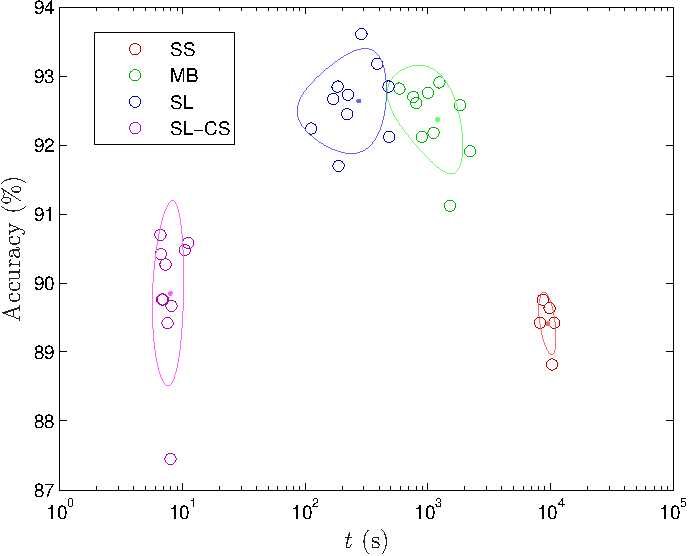
\includegraphics[width=0.61\textwidth]{images/usps-acc-time}}
	  \subfigure[\texttt{magic}]{\label{fig:magic}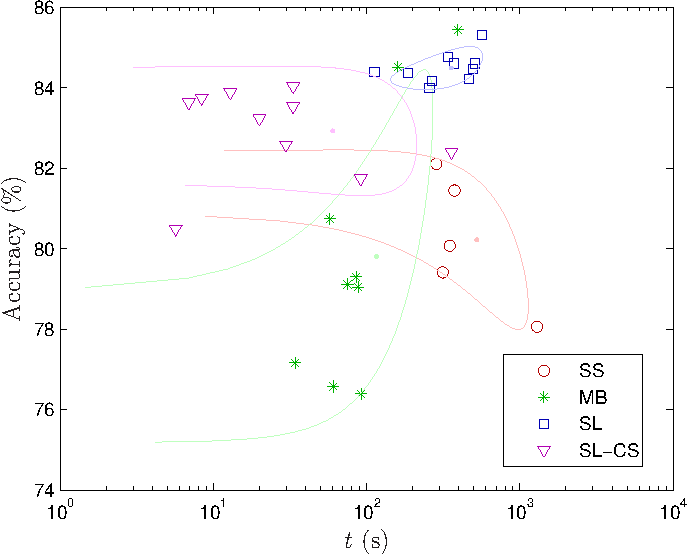
\includegraphics[width=0.61\textwidth]{images/magic-acc-time}}
	  \subfigure[\texttt{mnist}]{\label{fig:mnist}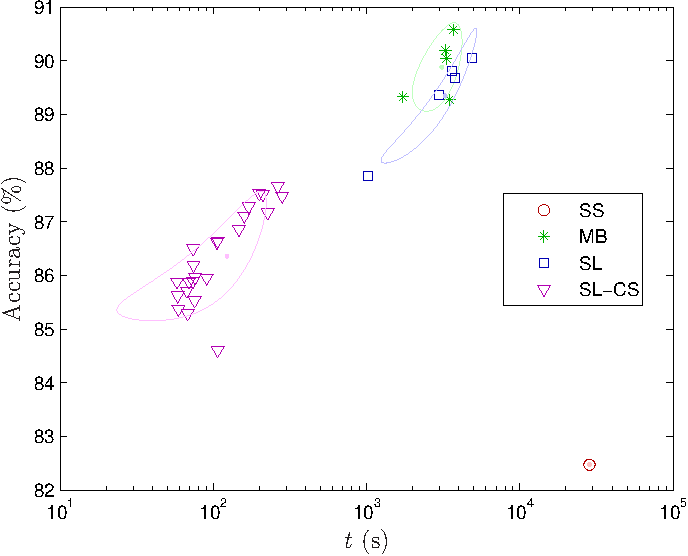
\includegraphics[width=0.61\textwidth]{images/mnist-acc-time}}
	  \caption{\small Time \textsl{vs.} accuracy plots on larger data sets.}
	  \label{fig:time-accuracy}
\end{figure}


\section{Approximate computations}
\label{sec:eval-nca-approx}

For KDE, demonstrate how $k$-d trees work better in low dimensions. Also show that if data has structure than the fraction of points visited for NN is lower. Contrast this with the case when we randomly initialize the projection matrix. We can arrive in such a scenario by initalizing with RCA.

Present fraction of points pruned.

Present results of KDE in terms accuracy. Argue that a reliable speeding can be achieved via a C implementation. We have investigated this using C code and found that is KDE is done fast enough.

%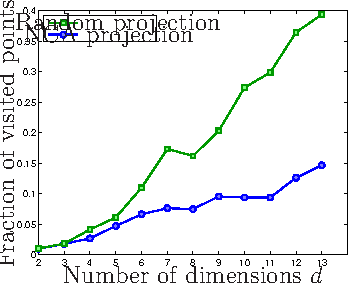
\includegraphics[width=\textwidth]{images/kd-tree-evol}

\subsection*{NCA with compact support kernels}
\label{subsec:eval-nca-cs}

\begin{figure}
	\centering
	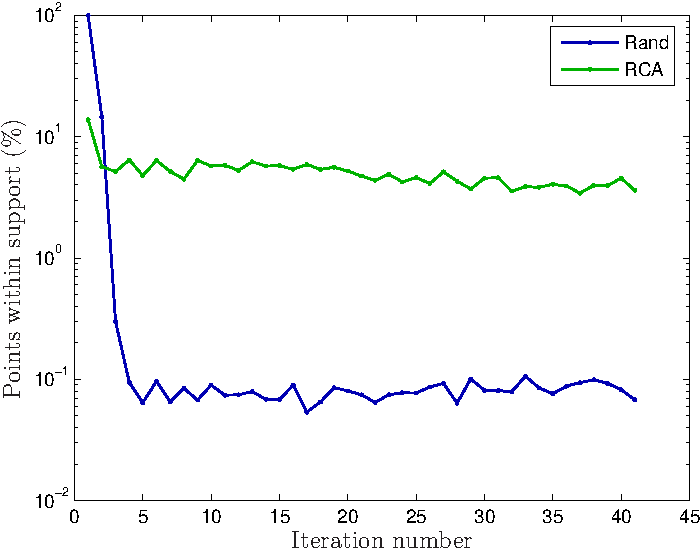
\includegraphics[width=0.6\textwidth]{images/nca-cs-nnzs}
\end{figure}

Demonstrate performance in terms of accuracy. Present also average fraction of points that lie outside the kernel. Test it on large data sets.

Point to Appendix for further experimentations.